\chapter{Implementation}
\label{chap:implementation}

\section{Instinct: the searchless engine}
\label{sec:instinct}

\subsection{Training data}
\label{subsec:training-data}
Instinct is trained on the dataset that Ruoss et al.~\cite{Ruoss2024} built for their searchless engine, released as ChessBench \cite{GoogleDeepMind2024}.
The positions in it are taken from games played on Lichess and annotated with Stockfish.
From this annotation, Ruoss et al.\ derive three training targets, each of which can drive a chess policy \cite{Ruoss2024}: the \emph{state-value} of a position (its win probability), the \emph{action-value} of every legal move in it (the win probability after that move), and the \emph{best action} for behavioural cloning.
ChessBench ships a separate dataset for each target.
Because every position yields one action-value per legal move, the action-value set is by far the largest: 15.32~billion action-values from 10~million games, against roughly 530~million state-values and best actions \cite{Ruoss2024}.
Producing it took about 8680 days of unparallelised Stockfish time \cite{Ruoss2024}, so the data was downloaded as released, not regenerated.

Instinct uses only the action-value data.
It is the default target in Ruoss et al., and it performed best in their comparison of the three, an advantage they attribute mainly to its much larger size \cite{Ruoss2024}.
Its training set is split into 2,148 shards \cite{GoogleDeepMind2024}, and Instinct is trained on the first 36 of them: 272~million samples, or about 1.7\,\% of the shards.
The validation set is 200,000 samples from the action-value test file.
The puzzle test set that comes with ChessBench is not used.
The cut-off was set by practical limits, not by experiment: the data had to fit on the laptop's disk, it had to fit into a container image small enough to upload to the GitHub Container Registry for training, and the conversion described below had to finish in reasonable time.

ChessBench stores its data in \texttt{.bag} files.
Each file holds the encoded records one after another, followed by an index table of 8-byte end offsets and a final 8-byte pointer to the start of that table \cite{GoogleDeepMind2024}.
An action-value record decodes to a position in \ac{FEN}, a move in \ac{UCI} notation and the move's win probability.
A conversion script, run in parallel across all \ac{CPU} cores, tokenises each position and move and writes the result to NumPy arrays: 72 unsigned 16-bit tokens per sample and the win probability as a 32-bit float.
For the training set, this gives a 37\,GB token array and a 1\,GB target array.

Ruoss et al.\ shuffled their dataset after annotation, because they train on individual positions, not whole games \cite{Ruoss2024}.
The shards can therefore be read in their stored order without reshuffling.
Instinct makes a single pass over the training set, so every sample is seen exactly once.

\subsection{Encoding board and move as tokens}
\label{subsec:encoding}

Instinct's transformer takes a sequence of 72 tokens: 71 describe the position and the last one is the candidate move.
Table~\ref{tab:tokens} lists the parts.

\begin{table}[htbp]
  \centering
  \caption{Instinct's 72-token input and the number of distinct tokens each part can take.}
  \label{tab:tokens}
  \begin{tabular}{lrr}
    \toprule
    Part & Tokens & Distinct values \\
    \midrule
    Squares a8 to h1      & 64 & 13 \\
    Side to move          & 1  & 2 \\
    Castling rights       & 4  & 5 \\
    En passant square     & 1  & 17 \\
    Half-move clock       & 1  & 28 \\
    Move                  & 1  & 1,968 \\
    \midrule
    Total                 & 72 & 2,033 \\
    \bottomrule
  \end{tabular}
\end{table}

The board is read rank by rank from a8 to h1, as in a \ac{FEN} string \cite{Ruoss2024}, with one token per square: one of the six white pieces, one of the six black pieces, or empty.
The side to move follows, then one token for each of the four castling rights, each holding either its right or a shared \emph{none} token.
The en passant token names one of the 16 squares on the third or sixth rank, or none.
Python-chess stores the \emph{potential} en passant square and provides \texttt{has\_legal\_en\_passant()} to test whether a capture there is actually possible \cite{pythonchess}.
Instinct sets the token only when that test passes, so it appears only when an en passant capture is a legal move.

The last state token is the half-move clock, the number of half-moves since the last capture or pawn move \cite{pythonchess}.
It is included on the assumption that Stockfish, which annotated the data \cite{Ruoss2024}, takes the clock into account, so that the same board can carry a different win probability depending on it.
Values from 0 to 19 each have their own token.
Above that the clock is bucketed in tens (20--29 up to 80--89), with one last token for 90 and more, which gives 28 tokens.
The buckets were chosen because high values are rare: in the training data, only 0.21\,\% of samples have a clock above 19.
The full-move number, which Ruoss et al.\ encode \cite{Ruoss2024}, is left out, because it only records how long the game has lasted.

Moves are written in \ac{UCI} notation, for example \texttt{e2e4}.
As in Ruoss et al., the move vocabulary is the alphanumerically sorted list of all 1,968 moves that can occur in a game, and a move's index in this list is its token \cite{Ruoss2024}.
Instinct rebuilds this list in code from all queen-direction and knight moves from every square plus the pawn promotions, which gives the same 1,968 moves.
Move tokens are numbered after the 65 state tokens, so the whole input shares one vocabulary of 2,033 tokens.

This encoding differs from that of Ruoss et al. They pad the \ac{FEN} string to a fixed 77 characters and use each character's ASCII code as a token \cite{Ruoss2024}, spelling the en passant square, the half-move clock and the full-move number character by character \cite{Ruoss2024}.
Instinct was trained twice, once with each of two encodings.
The first model, v1, also reused \ac{FEN} characters, so some of its tokens had two meanings: \texttt{b} stood for a black bishop and for black to move, \texttt{K} for the white king and for a castling right.
The second, v2, uses the encoding described above, which gives every token exactly one meaning and encodes each field as a single token.

Each token is mapped to a learned 256-dimensional embedding.
Since the input always has the same length, a learned positional embedding of $72 \times 256$ is added to it, as in Ruoss et al.\ \cite{Ruoss2024}.
The sum is the input to the transformer described next.
Figure~\ref{fig:instinct-forward} shows the whole path from position and move to win probability.

\subsection{Model architecture}
\label{subsec:architecture}

Instinct's network is a standard transformer encoder, built with the \texttt{nn.\allowbreak TransformerEncoder} class of PyTorch \cite{pytorch}.
It has 8 layers with 8 attention heads each, an embedding dimension of 256 and a feed-forward block that widens each token's vector to 1,024 and projects it back to 256.
Dropout is switched off.
Ruoss et al.\ describe the same network as a ``decoder-only transformer without causal masking'' \cite{Ruoss2024}.
Without the causal mask, every token can attend to every other token, as in an encoder \cite{Vaswani2017}, so this thesis calls it encoder-only.
Instinct generates nothing: the whole position is given at once, and there are no later tokens to hide.

Each layer follows the original transformer \cite{Vaswani2017}, which is what PyTorch's \texttt{nn.\allowbreak TransformerEncoderLayer} implements \cite{pytorch}.
Instinct keeps the layer's defaults, \ac{ReLU} as the activation and layer normalisation after each sub-layer \cite{pytorch}.
Ruoss et al.\ use SwiGLU in place of \ac{ReLU} \cite{Ruoss2024}, so the activation differs.
PyTorch's built-in layer offers \ac{ReLU} and GELU as named activations \cite{pytorch}; SwiGLU is not among them.

The input is the 72 embedded tokens.
Because attention runs in both directions, the output vector at each position can draw on the whole board.
Only the vector at the last position, the move token, is passed on: a linear layer maps it to 128 logits, and a softmax turns them into a probability distribution over 128 bins.
As in Ruoss et al., the bins split the range of win probabilities from 0 to 1 into equal intervals \cite{Ruoss2024}, and the move's win probability is the expected value of this distribution \cite{Ruoss2024}, with each bin represented by its centre.

Attention in this network relates the squares of a single position to each other.
The input holds no earlier positions, so the attention is spatial, not temporal.
Ruoss et al.\ do not say why a transformer suits chess; this reading is the author's own.

\begin{figure}[htbp]
  \centering
  \begin{tikzpicture}[flowchart, node distance=10mm and 11mm,
    dims/.style={above, gray, font=\scriptsize, inner sep=1.5pt}]
  \node[data] (in) {Position and\\candidate move};
  \node[process=29mm, right=of in] (tok) {Tokenise:\\71 state + 1 move};
  \node[process=29mm, right=of tok] (emb) {Token + positional\\embedding};
  \node[process=29mm, right=of emb] (enc) {8 encoder layers\\8 heads, FF 1,024};
  \node[process=29mm, below=of enc] (last) {Vector at the\\move token};
  \node[process=29mm, below=of emb] (head) {Linear layer and\\softmax, 128 bins};
  \node[process=29mm, below=of tok] (ev) {Expected value\\over the bin centres};
  \node[data] at (ev -| in) (out) {Win probability\\of the move};

  \draw[->] (in) -- (tok);
  \draw[->] (tok) -- node[dims] {72} (emb);
  \draw[->] (emb) -- node[dims] {$72{\times}256$} (enc);
  \draw[->] (enc) -- node[dims, right] {$72{\times}256$} (last);
  \draw[->] (last) -- node[dims] {256} (head);
  \draw[->] (head) -- node[dims] {128} (ev);
  \draw[->] (ev) -- (out);
\end{tikzpicture}

  \caption{Instinct's forward pass for one position and one candidate move, with the shape of the data on each arrow.}
  \label{fig:instinct-forward}
\end{figure}

Ruoss et al.\ train three sizes, from 8 layers with an embedding dimension of 256 up to 16 layers with 1,024 \cite{Ruoss2024}, the largest with roughly 270 million parameters \cite{Ruoss2024}.
Instinct deliberately copies the smallest one, which they list as 9M \cite{Ruoss2024}.
Two limits set this.
Training had to stay cheap, on a single rented \ac{GPU} overnight, and the finished model has to choose its moves within the time that the requirements allow.

Counted in code, Instinct has 6,889,856 parameters, about 26\,MB of weights.
The 8 layers hold 6.32 million of them, 4.20 million in their feed-forward blocks.
The token embeddings add 520,448 ($2{,}033 \times 256$), the positional embedding 18,432 and the output layer 32,896.
The gap to 9M could come from a different feed-forward width, which Ruoss et al.\ do not state, or from their use of SwiGLU instead of \ac{ReLU}.

\subsection{Training}
\label{subsec:training}

Instinct learns the win probability of a move as a classification over the 128 bins.
For each sample, the target win probability $p$ is mapped to the index of its bin, $\lfloor 128\,p \rfloor$, with $p = 1$ placed in the last bin, and the loss is the cross-entropy between the network's softmax over the bins and this one-hot target.
Ruoss et al.\ train with the same loss on the same one-hot bins \cite{Ruoss2024}.

The optimiser is AdamW.
Instinct sets only the learning rate, a fixed $3 \times 10^{-4}$ with no schedule, and keeps PyTorch's other defaults, including a weight decay of 0.01 \cite{pytorch}.
Batches hold 1,024 samples.
Ruoss et al.\ train their main models with Adam at a learning rate of $10^{-4}$ and a batch size of 4,096, and their smaller ablation runs with a batch size of 1,024 and a learning rate of $4 \times 10^{-4}$ \cite{Ruoss2024}.
Instinct follows the ablation setup: a smaller batch needs less \ac{GPU} memory, so it fits on a cheaper \ac{GPU}, and the smaller setup was expected to train in less time.
Its learning rate of $3 \times 10^{-4}$ is slightly lower than the ablation's; this difference was not tested.

Both training runs, v1 and v2, used the same data, hyperparameters and number of steps; only the encoding differed.
Training is a single pass over the 272~million training samples, which at 1,024 samples per batch gives 266,296 steps.
Ruoss et al.\ train for 10~million steps at a batch size of 4,096, or 2.67 epochs \cite{Ruoss2024}.
Every 1,000 steps, the loss on the 200,000 validation samples is computed and a checkpoint is saved, so an interrupted run can resume.
The model kept at the end is the one with the lowest validation loss, not the last one.
In both training runs this was the checkpoint at step 264,000, close to the end, so the choice made little difference in practice.

Training ran on a single rented \ac{GPU}.
Training on the author's laptop, an Apple M1, was not practical, so the converted data was packed into a container image and run on an NVIDIA RTX 3090 with 24\,GB of memory, rented from vast.ai for about \$0.20 per hour.
The first run took 7.5 hours and cost about \$1.50.
Ruoss et al.\ trained each of their three models, from 9M to 270M parameters, on 128 \acp{TPU} (V5) \cite{Ruoss2024}.

\subsection{Move selection}
\label{subsec:move-selection}

Instinct chooses its move as Ruoss et al.\ do: it evaluates every legal move in the current position and plays the one with the highest expected action-value \cite{Ruoss2024}.
Each legal move is tokenised together with the position, and all of them pass through the network as one batch.
This gives one win probability per legal move, and the move with the highest one is played.
There is no search beyond this single evaluation.

Ruoss et al.\ describe two weaknesses of this policy.
The first is ``indecisiveness in the face of overwhelming victory'' \cite{Ruoss2024}: in a very strong position, several moves end up in the top bin, so the engine picks among them almost at random instead of following one plan that finishes the game.
The second is that it cannot see a threefold repetition coming, because its input holds only the current position and no game history \cite{Ruoss2024}.
Together, the two let a won game end in a draw: the engine shuffles between moves that all look winning until a position occurs for the third time.
v1 and v2 both did this.
Ruoss et al.\ work around it in two ways.
They set the win probability of any move that would trigger a threefold repetition to 0.5, and when all of the top five moves score above 0.99, they check the position with Stockfish and play Stockfish's choice among those moves \cite{Ruoss2024}.

Instinct uses a rule of its own instead.
It was added after the second training run and leaves the network unchanged.
After the network has scored the legal moves, each move is played on the board in turn, and python-chess checks whether the game would then be over.
A move counts if it gives checkmate, if it ends the game in a draw, for example by stalemate, or if it lets the opponent claim a draw by threefold repetition or the fifty-move rule \cite{pythonchess}.
Every move that ends the game or allows a claim in this way is scored by its true result instead of the network's estimate: 1.0 for checkmate and 0.5 for any draw.
The board used for this check is the whole game, replayed from the moves the engine receives over \ac{UCI}, so the history that the network never sees is available here.
Figure~\ref{fig:move-selection} shows the whole selection.

\begin{figure}[htbp]
  \centering
  \begin{tikzpicture}[flowchart, node distance=6mm and 10mm]
  \node[data, minimum width=56mm] (in) {Start position and the moves so far,\\received over \acs{UCI}};
  \node[process=50mm, below=of in] (board) {Replay the moves on a board};
  \node[process=50mm, below=of board] (net) {Score every legal move with\\the network, all in one batch};
  \node[process=50mm, below=8mm of net] (try) {Try the move on the board};
  \node[decision, below=of try] (mate) {Checkmate?};
  \node[decision, below=of mate] (draw) {Drawn, or draw\\claimable?};
  \node[process=50mm, below=of draw] (keep) {Keep the network's estimate};
  \node[process=22mm, right=of draw] (half) {Score 0.5};
  \node[process=22mm] at (mate -| half) (one) {Score 1.0};
  \node[decision, below=of keep] (next) {Another legal\\move?};
  \node[process=50mm, below=of next] (best) {Choose the move with\\the highest score};
  \node[data, minimum width=56mm, below=of best] (out) {Chosen move,\\sent over \acs{UCI}};

  \draw[->] (in) -- (board);
  \draw[->] (board) -- (net);
  \draw[->] (net) -- (try);
  \draw[->] (try) -- (mate);
  \draw[->] (mate) -- node[branch] {no} (draw);
  \draw[->] (draw) -- node[branch] {no} (keep);
  \draw[->] (mate) -- node[branch] {yes} (one);
  \draw[->] (draw) -- node[branch] {yes} (half);
  \draw[->] (keep) -- (next);
  \draw (one.east) -- ++(4mm,0) coordinate (bus);
  \draw (half.east) -- (half.east -| bus);
  \draw[->] (bus) |- ($(keep.south)!0.5!(next.north)$);
  \draw[->] (next.west) -- node[branch, swap] {yes} ++(-8mm,0) |- (try.west);
  \draw[->] (next) -- node[branch] {no} (best);
  \draw[->] (best) -- (out);

  \node[group, fit=(try) (mate) (draw) (keep) (one) (half) (bus) (next),
    label={[anchor=north east, gray, inner sep=4pt]north east:for every legal move}] {};
\end{tikzpicture}

  \caption{Instinct's move selection: the network scores every legal move, and a move that mates or allows a draw is scored by its true result.}
  \label{fig:move-selection}
\end{figure}

Two consequences follow from the scores.
The network's estimate can never reach 1.0, because the highest bin centre is 0.996, so a mate in one is always played when there is one.
In a won position, a move that allows a draw scores 0.5 and loses to any move the network rates higher, so Instinct plays something else.
Compared with the workarounds of Ruoss et al., the rule covers the fifty-move rule and the game-ending draws as well as the threefold repetition, and it needs no second engine.
How much the rule helps is measured in the evaluation.

The rule also works in the other direction.
When every move scores below 0.5, a move that ends the game in a draw or lets one be claimed scores highest, so in a lost position Instinct takes a draw when one is available.

Instinct's move selection contains no randomness: the same game always leads to the same move.
Two games that start with the same moves would therefore be identical, so the engine tournament in the evaluation starts its games from a book of different openings.

\subsection{Deployment}
\label{subsec:deployment}

Instinct runs as an ordinary chess engine behind the \ac{UCI}, in which ``all communication is done via standard input and output with text commands'' \cite{uci}.
The engine tournament in the evaluation, The Bishop and a Lichess bot account all use it this way.
Before every move, the engine receives the start position and every move played so far \cite{uci}, and it rebuilds the board from them.
This is where the rule from the previous subsection gets the game history that the network never sees.
Time controls are ignored: with no search, Instinct does the same work on every move, one batch through the network.

\section{The Bishop: hardware and calibration}
\label{sec:bishop-hardware}

\subsection{Hardware setup}
\label{subsec:hardware}

The Bishop moves the pieces with a Franka robot arm and its standard gripper, the Franka Hand.
A PC controls both over Ethernet through franky, a Python library built on Franka's C++ library libfranka \cite{franky}, and commands the arm with Cartesian poses.
To grasp a piece, the hand closes to 15\,mm with a force of 20\,N; to release it, the hand opens to 20\,mm.

The camera is a USB webcam on the arm's wrist, which records at $1280 \times 720$ pixels.
It is mounted there because that is how the lab's setup provides it.
The camera's autofocus runs while the opponent lines up the viewing pose, and it is locked once the pose is set, because refocusing would change the image geometry that the calibration assumes.

The board is printed on three A4 sheets taped together, with an AprilTag at each corner.
A4 prints on any office printer, and three sheets side by side make a strip of $630 \times 297$\,mm: wide enough for the board in the middle and room on both sides of it, and wide like the camera's 16:9 image.
The configuration holds the dimensions of the board's design: 35\,mm squares, 15\,mm tags, and tag centres $589.5 \times 267$\,mm apart.
Every print comes out slightly different, so for the lab's board these values were measured on the print and changed locally.
The area beside the board, on both sides and inside the tags, is the parking area, where captured pieces are put.

The pieces are 34 3D-printed discs, 30\,mm across, each with a raised square about 15\,mm wide on top.
The square's top face, 6\,mm above the board, carries the piece's icon, printed in a colour that contrasts with the disc: white discs for one side, dark blue discs for the other.
Two spare queens, one per side, come on top of the full set of 32 so that a pawn can be promoted.
These pieces replaced an earlier design whose icons were too small and too alike to be told apart.

\subsection{Camera and hand-eye calibration}
\label{subsec:calibration}

Two calibrations link what the camera sees to where the arm moves.
The camera's intrinsic parameters, a $3 \times 3$ camera matrix and five lens distortion coefficients, turn a pixel into a ray through the camera's centre.
The hand-eye calibration gives the camera's pose relative to the arm's end effector, the frame at the gripper, as a $4 \times 4$ transformation matrix.
Combined with the end-effector pose that the arm reports, it places the camera, and with it everything the camera sees, in the robot's base frame.

Both come from the lab's calibration program rather than from a procedure written for The Bishop.
The results are stored as constants in the configuration.
Like the board dimensions, the repository holds placeholder values, and the lab's values are set locally.

The intrinsics are used wherever a pixel meets a physical length: to estimate the board's pose from the AprilTags, and to turn the pixel at a detected piece's centre into a point on the board.
The hand-eye matrix is used only when the viewing pose is set.
Once the opponent has lined it up, The Bishop reads the end-effector pose and multiplies it by the hand-eye matrix, which gives the camera's pose in the base frame.
The arm returns to exactly this pose before every look at the board, so the camera's pose stays valid until the viewing pose is set again.

\subsection{Board pose from AprilTags}
\label{subsec:board-pose}

The Bishop finds the board in the image through the four AprilTags at its corners.
They come from the 16h5 family, and OpenCV's ArUco module \cite{opencv} detects them in each camera frame.
The detector refines each tag's corners with OpenCV's AprilTag method.
Each tag carries its own ID, 0 to 3, so every detected corner can be matched to its known place on the board.
If any of the four tags is missing from the image, the board counts as not visible: The Bishop does not estimate the pose from fewer tags but asks the opponent to line up the viewing pose again.

Positions on the board are expressed in the board frame.
Its origin is the centre of the board, its $x$ axis points from the h-file towards the a-file, its $y$ axis from the eighth rank towards the first, and its $z$ axis points up out of the board.
The tag corners have fixed coordinates in this frame, taken from the configuration: each tag's centre lies at $(\pm 294.75, \pm 133.5)$\,mm, half the tag span from the origin, and its corners 7.5\,mm from the centre along each axis, all at $z = 0$.

OpenCV's \texttt{solvePnP} takes the 16 tag corners, their coordinates in the board frame and their pixels in the image, and estimates the board's pose relative to the camera.
Using the camera's intrinsics, its default iterative method finds the pose that minimises the reprojection error, the sum of squared distances between where the corners appear in the image and where the estimated pose projects them \cite{opencv}.
The four tags are spread across the board, so the 16 corners lie far apart.
The result is the $4 \times 4$ transformation ${}^{\mathrm{cam}}T_{\mathrm{board}}$ from the board frame into the camera frame.
It is estimated again at every look at the board, so if the board is nudged between two looks, the next transfer follows it.

The Bishop plans every transfer in the board frame.
Only when the arm is sent to a pose $p$ is that pose carried into the robot's base frame, through the board's pose in the camera frame and the camera's pose in the base frame from the viewing pose and the hand-eye matrix:
\begin{equation}
  {}^{\mathrm{base}}T_{p}
  = {}^{\mathrm{base}}T_{\mathrm{cam}} \,
    {}^{\mathrm{cam}}T_{\mathrm{board}} \,
    {}^{\mathrm{board}}T_{p}.
\end{equation}
The centre of a square follows from its file $f$ and rank $r$, both counted from 0 (the a-file and the first rank), and the square size $s$:
\begin{equation}
  x = (3.5 - f)\, s, \qquad y = (3.5 - r)\, s, \qquad z = 0.
\end{equation}
The square centres lie at indices 0 to 7 along each axis, and the board's centre lies halfway between them, at 3.5.
Subtracting the index from 3.5 therefore puts the origin at the centre of the board, with the a-file and the first rank on the positive side, as the axes require.
The reverse mapping takes a point on the board to the square it lies in.
A point outside the $8 \times 8$ squares maps to no square, and this is how The Bishop recognises a parked piece.

\section{The Bishop: vision pipeline}
\label{sec:bishop-vision}

\subsection{Design history}
\label{subsec:design-history}

The vision pipeline went through three designs.
The first used a single \ac{YOLO} segmentation model to find each piece and tell which piece it was in one step.
The pieces of the time carried small icons that looked much alike, so the model had to separate very similar pieces from a few pixels each, and it could not do so reliably.

The second design set learned recognition aside for the time being and put an AprilTag on every piece, one ID for each of the 12 combinations of piece type and colour.
It was meant as an interim solution: with recognition that worked, the rest of the system could be developed, and the vision could be revisited later.
The detector that finds the board's corner tags then also gave each piece's type, position and orientation, and it did so very reliably.
The aim was still to recognise the pieces themselves, so once the rest of the system worked, the tags were replaced as planned.

The current design returns to learning but splits the task in two.
The pieces were redesigned with a larger icon on a raised square, and two models share the work.
A \ac{YOLO} \ac{OBB} detector finds every icon in the image as a single class, without telling the icons apart.
A \ac{YOLO} classifier then names each icon from a crop cut along its box, as one of 12 classes.
Each model solves one easier problem: the detector only has to find where the icons are, and the classifier sees one icon at a time, large enough to make out its details.

\subsection{Dataset and labelling}
\label{subsec:dataset}

Both models are trained on one set of 30 photos, taken with a phone from above.
All of them show the same set of 12 pieces, one of each kind, or six of them in two of the photos.
The pieces lie on the printed board, on a plain light surface or on wooden floorboards, spread out or close together, in daylight or under a lamp that casts strong shadows.
The scenes were varied on purpose, so that the models would not come to rely on the board or on one kind of light.

Every icon was outlined in labelme \cite{labelme} as a four-point polygon and labelled with its colour and piece, such as \texttt{white\_knight}, which gives 348 labelled icons.
The photos are split before anything else is made from them: 24 photos with 282 icons for training and 6 photos with 66 icons for validation.
No photo in the validation set is therefore seen during training, by either model, although the pieces in it are the same.
For the detector, a script fits the minimum-area rotated rectangle around each polygon and writes its four corners, normalised by the image size, as one line in the \ac{YOLO} \ac{OBB} format.
All boxes get the single class \texttt{icon}, and the piece names are not used.

The classifier's data is generated from the same labels.
Each photo is first scaled down to the camera's resolution of $1280 \times 720$ pixels, which has the same aspect ratio.
For each icon, the rotated rectangle gives a square crop whose side is 1.25 times the rectangle's longer side.
The crop is rotated upright and scaled to $64 \times 64$ pixels.
At run time, the same cropping code cuts the crops along the detector's boxes, so the classifier sees crops made the same way in training and in use.
For the training set, each icon is cut six times: once exactly and five times with its centre shifted by up to 2 pixels, its size scaled by 0.9 to 1.15 and its angle turned by up to $7^\circ$, which imitates a detector box that sits slightly off.
Every crop is then saved in all four quarter turns, because a square box does not tell which side of the icon is up.
This gives 6,768 training crops and 264 validation crops, sorted into one folder per class, with about the same number of icons in each.

\subsection{Two-stage recognition}
\label{subsec:two-stage-recognition}

Both models are the smallest, nano versions of YOLO26 and are fine-tuned from the pretrained weights that Ultralytics publishes.
Both were trained with the Ultralytics library \cite{ultralytics} on the \ac{GPU} of the author's laptop, an Apple M1: the detector in about 45 minutes, the classifier in about six.

The detector is trained on the full photos at an input size of 1280 pixels, the width of the camera image, so that the icons are not scaled down any further.
Most settings are the library's defaults.
Apart from the input size, three are changed.
The images are rotated at random by up to $180^\circ$, because an icon can lie on the board at any angle.
They are scaled by at most 30\,\% instead of 50\,\%, since the camera always looks at the board from the same height and the icons vary little in size.
Training runs for up to 200 epochs and stops early once the validation score has not improved for 50 of them.
The run stopped after 155 epochs, and the weights kept are those of epoch 105, which scored best on the validation photos.

The classifier is trained on the $64 \times 64$ crops at that same size, for 25 epochs.
Its augmentation is cut back so that it does not create images that never occur at run time.
Horizontal flips are turned off, because a mirrored icon does not exist on the real pieces.
Random erasing and the automatic augmentation policy are turned off as well, and the random scaling is reduced to 15\,\%.
Rotation is left off: the quarter turns and the small angle jitter of the crops already cover the angles a crop can have.

At run time, both models run on every camera frame in which the board is found.
The detector returns a rotated box for every icon it finds with a confidence of at least 0.25, the library's default.
The false positives among these boxes are then removed, as described in the next subsection, and each remaining box is cut into a crop, upright and $64 \times 64$ pixels in size, from a copy of the frame taken before anything was drawn on it.
All crops of a frame go to the classifier in one batch, and each icon is given the class with the highest score.
The classifier has no threshold and always names one of the 12 classes, so a wrong name is not caught here but by the checks on the board state that follow.

\subsection{From detections to board state and move}
\label{subsec:board-state}

Every box the detector returns is first given a position on the board.
The box's centre is the centre of the icon, but the icon lies on the top face of the piece, 6\,mm above the board.
Projected straight onto the board plane, it would land beside the piece's footprint, and the further from the middle of the image the piece stands, the further off it would be.
The Bishop therefore removes the lens distortion from the centre pixel and turns it into a ray from the camera.
Using the board's pose from the tags, the ray is cut with a plane parallel to the board at the height of the icons, 6\,mm, and the point where it hits is moved straight down onto the board.
This point, in the board frame, is the centre of the piece's footprint.
The piece's yaw is taken from the box's angle in the image.
Because the icon is square, this angle is only known up to a quarter turn, which the motion planner takes into account when it grasps the piece.

With every detection in board coordinates, the false positives are removed in millimetres on the board plane.
A detection is dropped if its centre lies outside the rectangle bounded by the outer edges of the four tags: these were the detections on the bench around the board, the most common error in practice.
A detection is also dropped if its centre lies within 22.5\,mm of a tag's centre, the radius of a piece plus half a tag, because the detector sometimes took a corner tag for an icon.
The Bishop never parks a piece that close to a tag.
Only the detections that remain are cropped and classified, so each one becomes a piece with a class, a position, a yaw and the square it stands on.
A piece whose position lies outside the $8 \times 8$ squares has no square and counts as parked.

The pieces on squares, with the parked pieces left out, make up the detected position.
Before The Bishop accepts it, it makes two checks.
First, all 34 pieces must be found, parked ones included, so every piece taken off the board, a captured piece or a promoted pawn, has to lie in the parking area, where the camera can see it.
A piece that is hidden or not detected breaks this check, and so does a single false detection, which is why the filters above matter.
While the count is wrong, the display shows how many pieces are visible, and The Bishop keeps looking.
Second, after the opponent's turn, the new position must follow from the old one by a legal move.
The Bishop plays each legal move of the old position in turn with python-chess and compares only the placement of the pieces with the detected position.
If no move matches, the display shows ``Illegal move'' next to the detected board, and the opponent can correct the board and let The Bishop look again, or reset the game.
If a move matches, it is played on the game board, so the board holds the whole game, including the castling rights and en passant squares that the camera cannot see.
Captures, castling, en passant and promotions need no special cases, because the comparison covers every legal move: a pawn promotes when the opponent replaces it with a spare queen, or with another of their own pieces from the parking area.
At the start of a game and after each of The Bishop's own transfers, only the count is checked, since the board is then not the result of the opponent's move.
Figure~\ref{fig:vision} summarises a look at the board, from the viewing pose to the detected position.

\begin{figure}[htbp]
  \centering
  \begin{tikzpicture}[flowchart, node distance=6mm and 8mm]
  \node[process=44mm] (view) {Move the arm to the viewing pose};
  \node[data, below=12mm of view] (frame) {Camera frame};
  \node[decision, below=10mm of frame] (tags) {All four\\tags found?};
  \node[process=44mm, below=of tags] (pose) {Board pose from the tags};
  \node[process=44mm, below=of pose] (det) {Detect the icons and\\place them on the board};
  \node[process=44mm, below=of det] (filter) {Drop the false positives};
  \node[process=44mm, below=of filter] (cls) {Classify the icons};
  \node[decision, below=of cls] (count) {All 34 pieces\\found?};
  \node[data, below=of count] (out) {Detected position, parked pieces\\and free parking spot};

  \node[process=30mm, left=of tags] (realign) {Opponent lines up\\the arm by hand};
  \node[decision] at (frame -| realign) (key) {Key?};
  \node[process=24mm] at (view -| realign) (save) {Save the\\viewing pose};
  \node[process=22mm, left=of key] (restore) {Arm moves to\\the saved pose};
  \node[process=24mm, right=of count] (show) {Show the piece\\count; opponent\\fixes the board};

  \draw[->] (view) -- (frame);
  \draw[->] (frame) -- (tags);
  \draw[->] (tags) -- node[branch] {yes} (pose);
  \draw[->] (pose) -- (det);
  \draw[->] (det) -- (filter);
  \draw[->] (filter) -- (cls);
  \draw[->] (cls) -- (count);
  \draw[->] (count) -- node[branch] {yes} (out);
  \draw[->] (tags) -- node[branch, swap] {no} (realign);
  \draw[->] (realign) -- (key);
  \draw[->] (key) -- node[branch] {space} (save);
  \draw[->] (key) -- node[branch, swap] {\texttt{g}} (restore);
  \draw[->] (restore) |- (realign);
  \draw[->] (save) -- (view);
  \draw[->] (count) -- node[branch] {no} (show);
  \draw[->] (show.east) -- ++(4mm,0) |- (view.east);
\end{tikzpicture}

  \caption{Looking at the board, from the viewing pose to the detected position, repeated until all four tags and all 34 pieces are found.
    The space key is offered only while all four tags are in view.
    The check that the position follows by a legal move is part of the game loop (Figure~\ref{fig:game-loop}).}
  \label{fig:vision}
\end{figure}

The same look at the board also finds a free spot in the parking area for the next piece The Bishop removes.
The spot is searched on a 2\,mm grid, column by column from the edge of the board outwards and on both sides of it, and the first point that is at least a piece's diameter plus 2\,mm away from every parked piece is used.
A parked piece keeps at least 20\,mm from the board's edge and 2\,mm clear of the tags.
If the parking area is full, The Bishop stops with an error.

\section{The Bishop: motion}
\label{sec:bishop-motion}

\subsection{Motion planner}
\label{subsec:motion-planner}

The motion planner turns a target position into movements of the arm.
During the game the target is the position after Instinct's move; after the game it is the start position.
The planner does not plan a whole move in advance.
It compares the detected position with the target square by square: a piece that stands on a square where the target has a different piece, or none, is surplus, and the piece the target has there is wanted.
From this difference the planner chooses a single transfer, one piece carried from where it stands to a square or to the parking area.
The arm then returns to the viewing pose, The Bishop looks at the board again, and the next transfer is planned from the new detection.
This repeats until no rule finds a transfer, which is the case once the detected position equals the target (Figure~\ref{fig:transfer-loop}).
Every transfer therefore starts from where the pieces really are, not from where an earlier plan expected them to be.

\begin{figure}[htbp]
  \centering
  \begin{tikzpicture}[flowchart, node distance=6mm and 10mm]
  \node[data] (in) {Target position};
  \node[subprocess=44mm, below=of in] (look) {Look at the board\\(Figure~\ref{fig:vision})};
  \node[decision, below=of look] (fill) {Empty square\\that can be filled?};
  \node[decision, below=of fill] (wrong) {Square held by\\a wrong piece?};
  \node[decision, below=of wrong] (surplus) {Surplus piece\\left?};
  \node[data, below=of surplus] (out) {No transfer left:\\the board matches the target};

  \node[process=44mm, right=of fill] (place) {Fill it with a matching piece:\\from a square before the\\parking area, nearest first};
  \node[process=44mm, minimum height=13mm] at (wrong -| place) (park) {Park that piece};
  \node[process=44mm] at (out -| place) (move) {Carry out the transfer};

  \draw[->] (in) -- (look);
  \draw[->] (look) -- (fill);
  \draw[->] (fill) -- node[branch] {yes} (place);
  \draw[->] (fill) -- node[branch] {no} (wrong);
  \draw[->] (wrong) -- node[branch] {yes} (park);
  \draw[->] (wrong) -- node[branch] {no} (surplus);
  \draw[->] (surplus) -| node[branch, pos=0.1] {yes} (park.south);
  \draw[->] (surplus) -- node[branch] {no} (out);
  \draw (place.east) -- ++(5mm,0) coordinate (bus);
  \draw (park.east) -- (park.east -| bus);
  \draw[->] (bus) |- (move.east);
  \draw[->] (move.south) -- ++(0,-5mm) -| ($(move.east -| bus) + (5mm,0)$) |- (look.east);
\end{tikzpicture}

  \caption{The motion planner's loop: after every look at the board, one transfer is chosen by three rules tried in order and carried out.
    On The Bishop's turn, the look made after the opponent's move serves as the first one.}
  \label{fig:transfer-loop}
\end{figure}

The transfer is chosen by three rules, tried in order.
First, an empty square that the target wants filled is filled with a piece of the wanted type and colour, taken from a surplus square or from the parking area.
A piece on the board is preferred, and among several, the one nearest to the square.
Second, if no empty square can be filled, the piece on a square that the target wants for a different piece is parked.
Third, any surplus piece that is left is parked.
No kind of move needs a rule of its own.
A capture parks the captured piece and then moves the capturing one, castling moves the king and the rook one after the other, and en passant moves the pawn and then parks the pawn it captured.
A promotion places a parked piece of the promoted type on the promotion square and then parks the pawn.
The same rules reset the board after a game, from any position.
Since the parked pieces are the only source, a promotion works only if such a piece is parked: the spare queen covers the first promotion to a queen on each side, and any further promotion needs a captured piece of that type.
If none is parked, the planner stops once no rule finds a transfer, and the promotion square stays empty.

A transfer is a fixed sequence of poses of the end effector.
They are computed in the board frame and turned into the robot's base frame with the board's pose from the last look and the camera's pose at the viewing pose.
Throughout, the gripper points straight down.
The hand opens, moves to 15\,mm above the piece's grasp pose, moves down to the grasp height of 5\,mm above the board, closes and moves back up.
It then moves to the same height above the target, moves down, opens and moves up again.
The target is the centre of a square, or the free spot in the parking area that the last look found.
At the grasp height the fingers close on the raised square, not on the disc, and while the piece is carried, its base is 15\,mm above the board, clear of the 6\,mm pieces it passes over.

The gripper also has to be turned so that its fingers meet two opposite faces of the raised square.
The square's angle is known from the detection, but only up to a quarter turn, so four angles of the gripper fit it equally well.
The planner takes the one closest to the gripper's angle at the viewing pose, so the wrist never turns more than $45^\circ$ away from it.
Turning the gripper is by far the slowest part of the arm's motion, so keeping the turn small shortens every transfer.
The piece is put down with its square aligned to the squares of the board, again in the quarter turn closest to the viewing pose.
Whether a target square is free is taken from the detected position, not from the measured positions of the pieces, and a piece is always put down at the centre of its square.

\subsection{Robot abstraction}
\label{subsec:robot-abstraction}

The motion planner does not control the Franka arm directly.
It goes through a small interface, \texttt{Robot}, with four operations: read the pose of the end effector, move the end effector to a pose, close the gripper and open it.
A pose is a $4 \times 4$ homogeneous matrix in the robot's base frame, in millimetres, the same form as the poses of the board and the camera.
\texttt{Robot} is an abstract class, so that The Bishop can work with any arm.
The one implementation so far, \texttt{FrankaEmika}, is for the Franka arm in the lab.
Each operation calls a method that the subclass implements, and wraps that call so that an error does not end the game: the operator display shows the error and waits for the opponent to press the space key, and the same call is then tried again.

\section{Integration: the game loop and operator display}
\label{sec:integration}

A single script, \texttt{play.py}, ties the parts together.
It runs the game loop (Figure~\ref{fig:game-loop}), asks the vision pipeline for the position, asks Instinct for a move, hands the target position to the motion planner and keeps the operator display up to date.

At start-up, the opponent lines up the viewing pose.
The display shows the live camera image, and the opponent can continue as soon as all four AprilTags are in view, or send the arm back to the viewing pose saved last time.
The Bishop then looks at the board, and the first game starts from the position it finds.
The opponent can set out the pieces by hand, or press \texttt{r} to have the arm set up the start position.
On its turn, The Bishop sends the game board to Instinct over \ac{UCI} with python-chess and gives the position after the returned move to the motion planner as the target, which carries out transfers until the detected position matches it.
On the opponent's turn, the opponent moves a piece by hand and presses the space key to end the turn.
The Bishop then looks at the board and accepts the new position once the two checks on it pass.
After every move, The Bishop asks python-chess whether the game is over.
Besides checkmate and the draws that end a game by themselves, such as stalemate, this includes the draws that a player could claim, by threefold repetition or the fifty-move rule; The Bishop claims them at once on behalf of both sides.
The display then shows the result, and once the opponent presses \texttt{r}, the motion planner resets the board to the start position and the next game begins.
The same key abandons a game and resets the board on any of the opponent's turns, and \texttt{q} quits The Bishop at any time.

The operator display is a single window (Figure~\ref{fig:canvas}).
Its top part shows a status line, such as ``Your turn'' or ``The Bishop's turn -- moving'', with the keys that are available at that moment listed below it.
Next to them are two diagrams of the board, drawn from the opponent's side: the position The Bishop expects, which is the game board or, during its own turn, the target, and the position it detected on its last look.
A king in check is marked in both.
The bottom part shows the camera image of the last look, with the box, centre and class of every detected piece and the free spot in the parking area drawn on it.
While the arm moves, the image also shows the pose the end effector is moving to as its three axes, with a dot when the gripper is closed, so the operator can see where the arm is going before it gets there.

\begin{figure}[htbp]
  \centering
  \begin{tikzpicture}[flowchart, node distance=6mm and 14mm]
  \node[terminal] (start) {Start};
  \node[subprocess=56mm, below=of start] (look0) {Look at the board\\(Figure~\ref{fig:vision})};
  \node[process=56mm, below=8mm of look0] (turn) {Opponent moves a piece by hand\\and presses a key};
  \node[decision, below=10mm of turn] (key) {Key?};
  \node[subprocess=56mm, below=of key] (look) {Look at the board\\(Figure~\ref{fig:vision})};
  \node[decision, below=of look] (legal) {Does a legal\\move match?};
  \node[process=56mm, below=of legal] (playopp) {Play the move on the game board};
  \node[decision, below=of playopp] (over1) {Game over?};
  \node[process=56mm, below=8mm of over1] (engine) {Instinct chooses a move over \acs{UCI};\\the position after it is the target};
  \node[subprocess=56mm, below=of engine] (transfer) {Carry out transfers until the\\board matches (Figure~\ref{fig:transfer-loop})};
  \node[decision, below=of transfer] (over2) {Game over?};

  \node[process=28mm, left=of legal] (illegal) {Show\\\enquote{Illegal move}};
  \node[subprocess=30mm, right=of key] (reset) {Reset the board to\\the start position\\(Figure~\ref{fig:transfer-loop})};
  \node[process=30mm] at (over1 -| reset) (result) {Show the result;\\wait for \texttt{r}};

  \draw[->] (start) -- (look0);
  \draw[->] (look0) -- (turn);
  \draw[->] (turn) -- (key);
  \draw[->] (key) -- node[branch] {space} (look);
  \draw[->] (key) -- node[branch] {\texttt{r}} (reset);
  \draw[->] (reset) |- (turn);
  \draw[->] (look) -- (legal);
  \draw[->] (legal) -- node[branch] {yes} (playopp);
  \draw[->] (legal) -- node[branch, swap] {no} (illegal);
  \draw[->] (illegal) |- (turn.west);
  \draw[->] (playopp) -- (over1);
  \draw[->] (over1) -- node[branch] {no} (engine);
  \draw[->] (over1) -- node[branch] {yes} (result);
  \draw[->] (engine) -- (transfer);
  \draw[->] (transfer) -- (over2);
  \draw[->] (over2) -| node[branch, pos=0.1] {yes} (result);
  \draw[->] (result) -- (reset);
  \coordinate (bus) at ($(illegal.west) + (-5mm,0)$);
  \draw[->] (over2.west) -- node[branch, swap, pos=0.1] {no} (over2.west -| bus) |- (turn.west);
\end{tikzpicture}

  \caption{The game loop: start-up, the opponent's turn, The Bishop's turn, the end of the game and the reset.
    The key \texttt{q}, which quits The Bishop at any time, is left out.}
  \label{fig:game-loop}
\end{figure}

\begin{figure}[htbp]
  \centering
  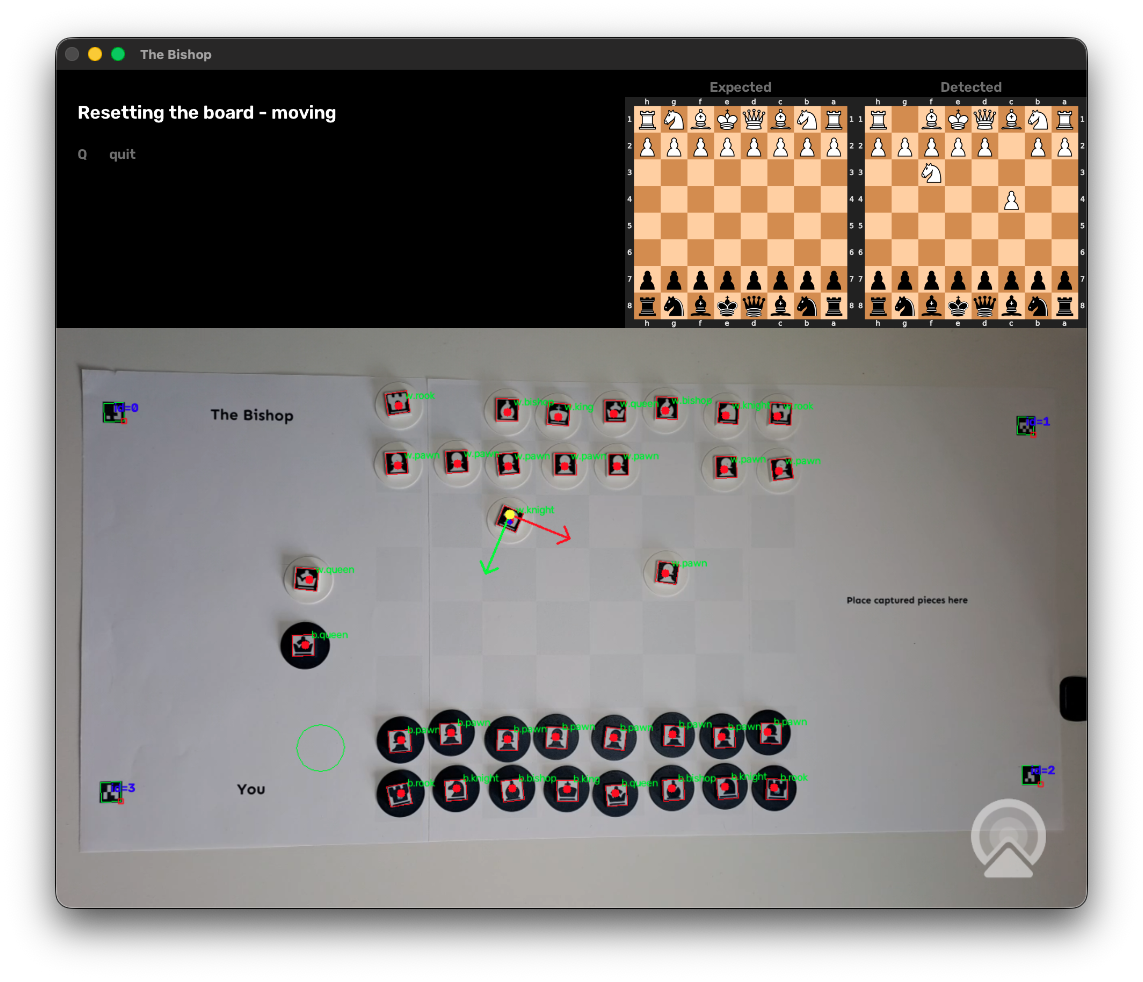
\includegraphics[width=0.9\textwidth]{figures/operator-display.png}
  \caption{The operator display during The Bishop's turn: the status line and the available keys, the expected and the detected board, and the camera image of the last look with the detected pieces, the free parking spot and the end effector's next pose.}
  \label{fig:canvas}
\end{figure}
